%%%%%%%%%%%%%%%%%%%%%%%%%%%%%%%%%%%%%%%%%%%%%%%%%%%%%%%%%%%%%%%%%%%%%%%
%% Related Work
\subsection{Physically Embedded Intelligent Systems - PEIS}
\label{sec:relatedwork-peis}

Ähnlich der Einleitung zu dieser Arbeit beschreiben auch Broxvall und Kollegen ihre Zukunftsvision von Robotern im sozialen und alltäglichen Umfeld. Im Fokus ihres Szenarios stehen dabei die unterschiedlichen Sensoren und Aktoren in einem intelligenten Gebäude, im Zusammenspiel mit Robotern. Dieses Zusammenspiel ist das zentrale Konzept der Arbeit von Broxvall und wird als PEIS-Ökologie bezeichnet. PEIS steht für Physically Embedded Intelligent Systems und umfasst die Kernkonzepte von künstlicher Intelligenz, allgegenwärtigem Rechnen und Robotik. Die Abbildung \ref{fig:sota-peis} zeigt die Überschneidung dieser Themenbereiche, sowie die Position, an der Broxvall und Kollegen ihre Arbeit sehen \citep{Saffiotti:2005:PEA:1107548.1107615}. Der Begriff Ökologie wird als Analogie zu dem Begriff aus der Biologie gesehen und soll das Zusammenspiel der einzelnen Agenten mit der Umgebung beschreiben.


\begin{figure}[H]
	\centering
	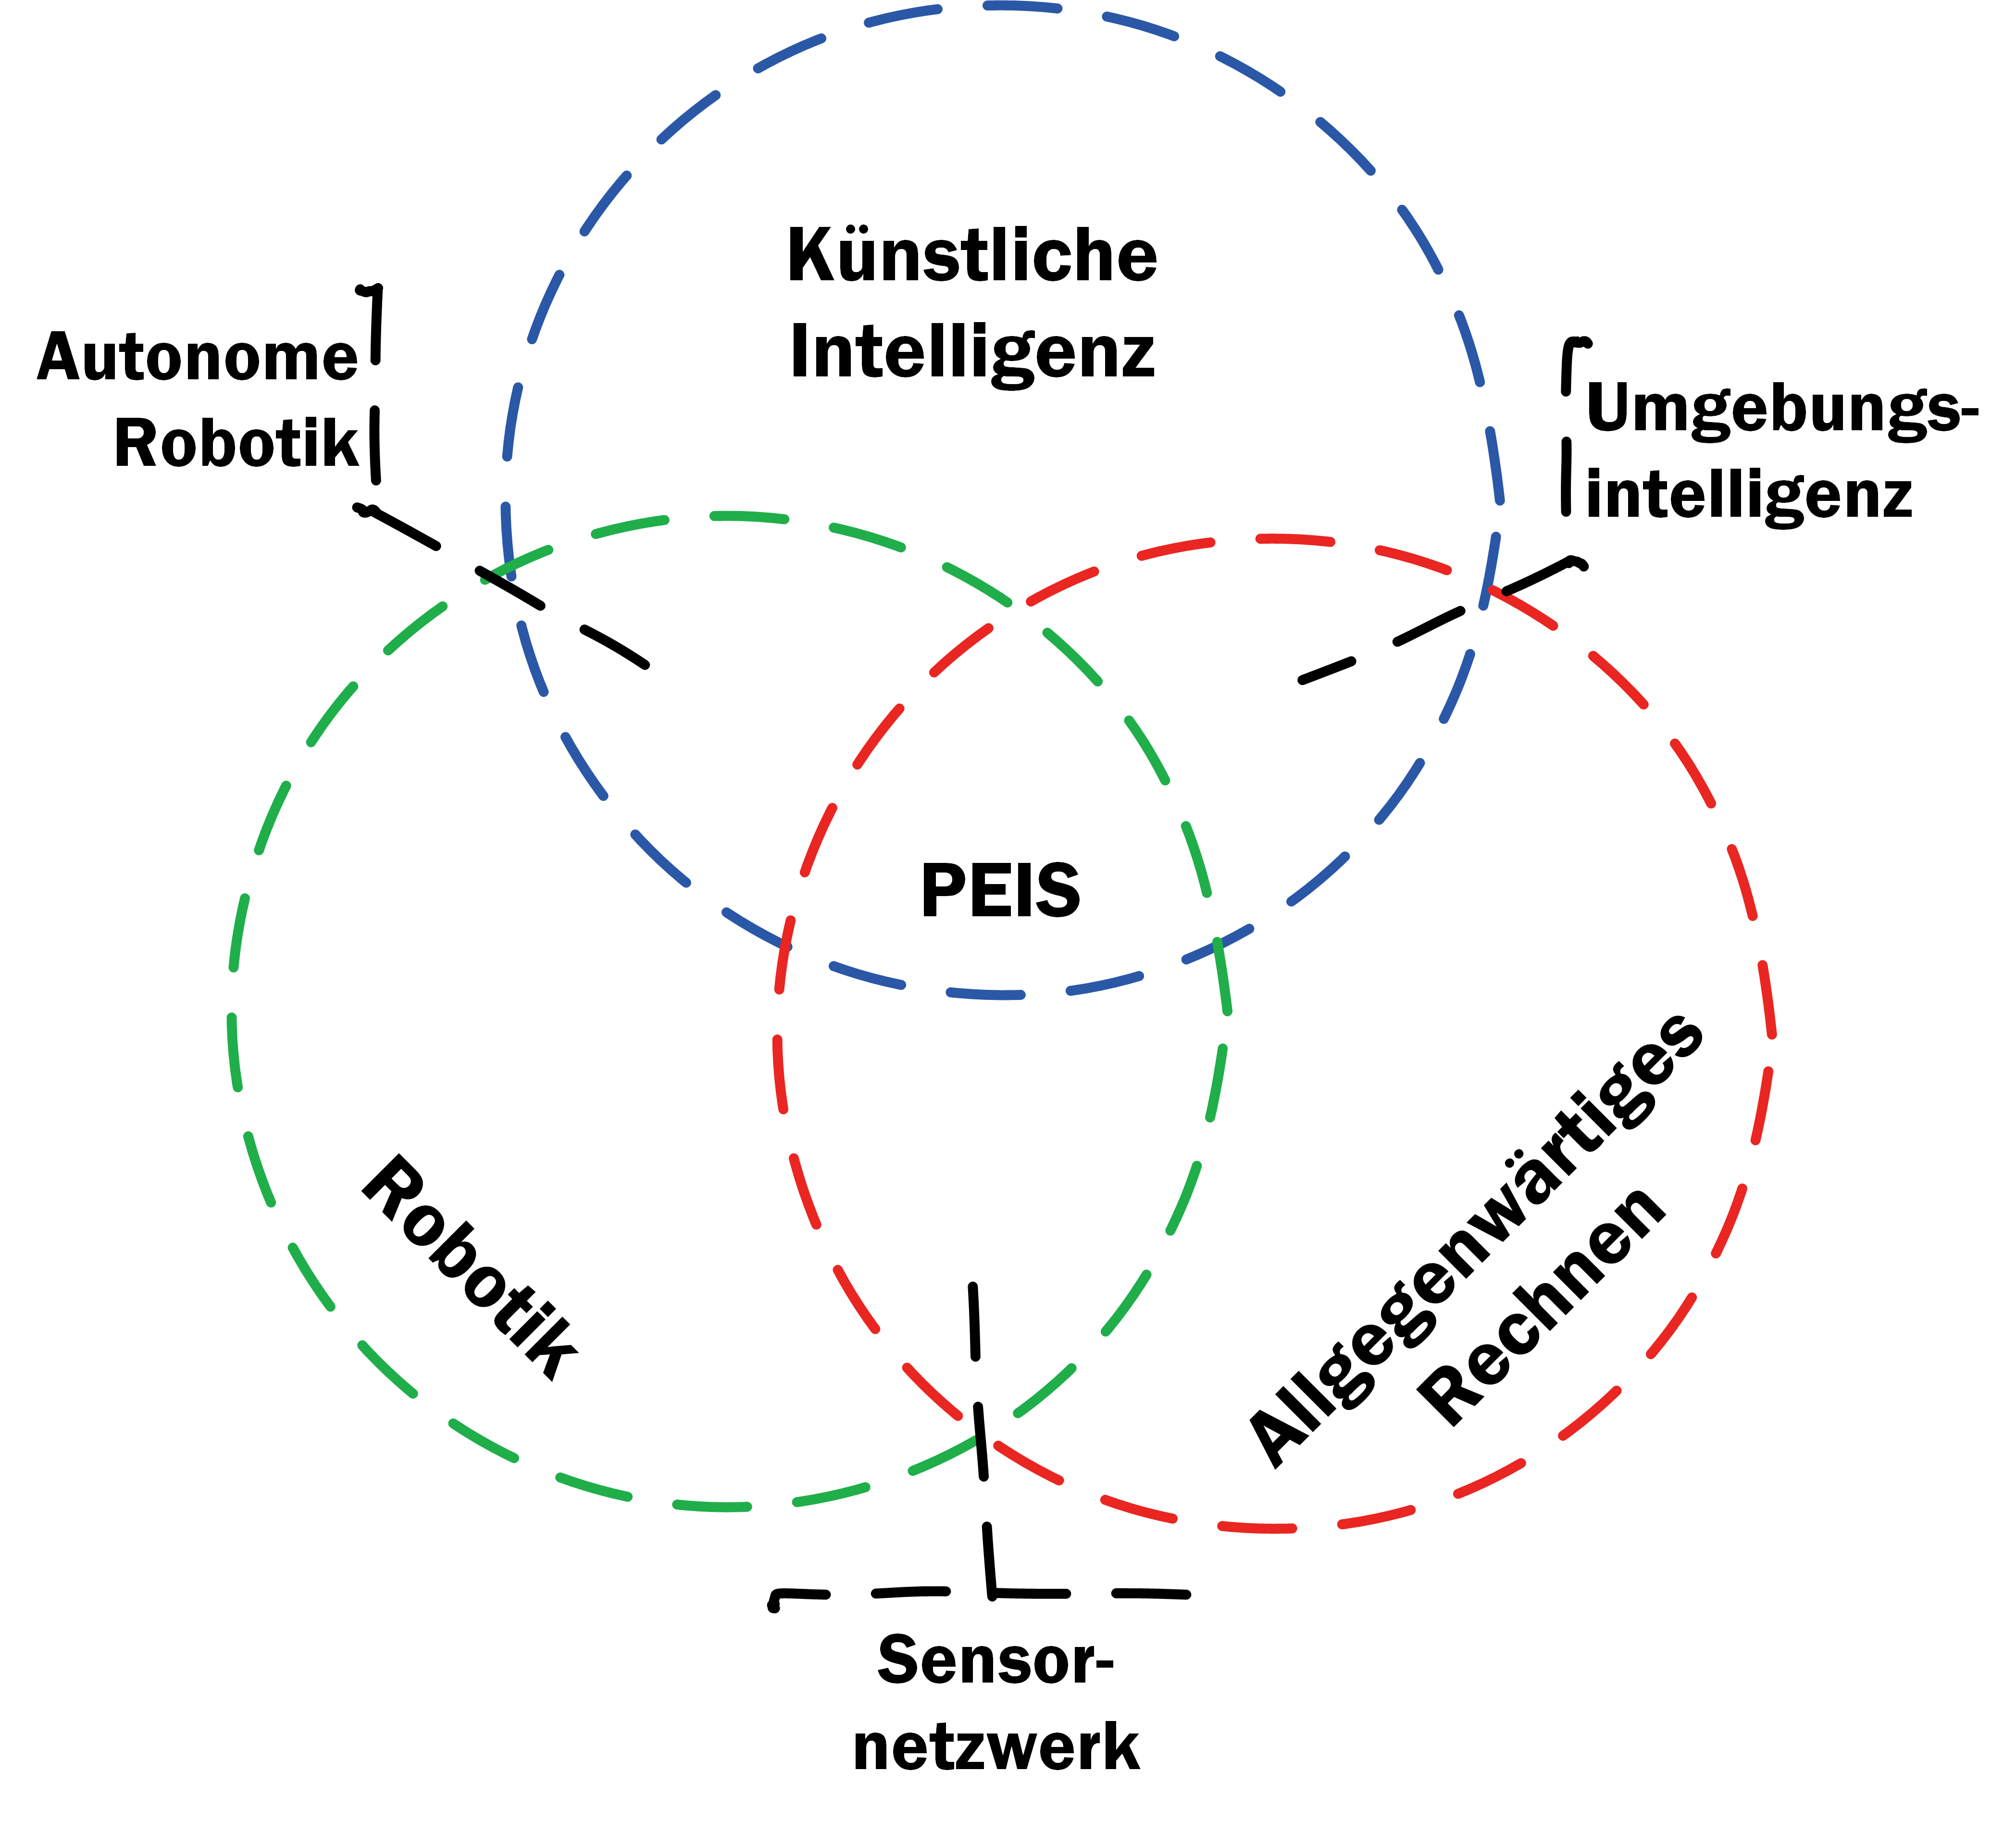
\includegraphics[scale=0.6]{fig/peis}   
	\caption[Kompetenzen PEIS]{PEIS liegt in den Schnittmengen mehrerer Kernkompetenzen. Bildquelle: \cite{Saffiotti:2005:PEA:1107548.1107615}}
	\label{fig:sota-peis}
\end{figure}


\subsubsection{Konzept}
Das Konzept der PEIS-Ökologie beruht auf drei Grundlagen (vergleiche \cite{Saffiotti:2005:PEA:1107548.1107615}). Zunächst wird die gleichmäßige Notation von PEIS (\textit{uniform notion of PEIS}) vorgestellt. Jedes technische Gerät ist eine mögliche PEIS-Komponente, wenn es über eine Recheneinheit und eine Kommunikationsschnittstelle verfügt, sowie mit der Umwelt interagieren kann. Dies betrifft sowohl Aktoren als auch Sensoren und reicht vom einfachen Toaster über den intelligenten Feuermelder bis zum komplexen Roboter. Das zweite zentrale Konzept ist das einheitliche Kommunikationsmodell (\textit{uniform communication model}). Dieses Modell realisiert die Dynamik eines PEIS. Zu jedem Zeitpunkt können sich neue PEIS-Komponenten anmelden und bestehende Komponenten das Modell verlassen. Das Modell ermöglicht eine einheitliche Kommunikation und versteckt die Heterogenität zweier PEIS-Komponenten unabhängig vom physikalischen Kommunikationsmedium. \citep{Saffiotti:2005:PEA:1107548.1107615} Die dritte Kernkompetenz ist das einheitliche Kooperationsmodell (\textit{uniform cooperation model}). Dabei beschreiben Broxvall und Kollegen die Verbindung funktionaler Komponenten. Diese Verbindung ermöglicht es jeder PEIS-Komponente Funktionen anderer PEIS-Teilnehmer anzufordern. Diese drei Konzepte repräsentieren die Stärke eines PEIS: Die Zusammenarbeit mehrerer unabhängiger Systeme. 

\subsubsection{Implementation}
\label{sec:peis-imple}
Neben dem Konzept der PEIS-Ökologie stellen Broxvall und Kollegen in ihrer Arbeit die Implementation einer PEIS-Ökologie vor. Dabei wird zunächst nur die Abstraktion der Robotersysteme, sowie der Umwelt angestrebt. Dazu werden funktionelle Aufgaben und physikalische Systeme getrennt und einander zugewiesen. So werden zum Beispiel Kameras und Lasersensoren für die visuelle Raumwahrnehmung, Saugroboter für die Hindernisbeseitigung und die Reinigung eingeteilt. Neben der Funktionalität müssen die PEIS-Komponenten Schnittstellen anbieten, damit andere PEIS-Komponenten die Funktionen anfordern können. Der nächste Schritt ist die Entwicklung des Kommunikationsmodells. Broxvall und Kollegen empfehlen die Verwendung eines Hybridmodells zwischen einem Event-basierten und einem Tuple-Space Modell. Diese Empfehlung lässt sich auf die Abbildung \ref{fig:sota-peis} zurückführen. Arbeiten in den Bereichen Umgebungsintelligenz (siehe dazu \cite{arregui2003stitch} und \cite{siegemund2004context}), Sensornetzwerke (siehe \cite{adjie1999design} und \cite{heidemann2001building}) sowie Robotik (\cite{caceres2003real}) setzen auf diese Kommunikationsmodelle, sowie auf die Hybridform. Für PEIS wird ein Eventbus-System ähnlich den ROS-Topics gefordert. Dieses ermöglicht das autonome An- und Abmelden von Komponenten. Das Tupel-Space-Modell kann für die PEIS-Ökologie simpel gehalten werden und wird von Broxvall und Kollegen mit der Form beschrieben:

{\tt <peisID, compID, key, val0, ..., valN>}

{\tt peisID} und {\tt compID} identifiziert dabei die PEIS-Komponente, sowie die innere logische Einheit. {\tt key} bezeichnet das Tupel selbst. Die dritte Komponente der Implementierung ist die Konfiguration der Ökologie. Diese beinhaltet alle Informationen über die Funktionalitäten des System, sowie die Verbindungen der einzelnen Komponenten untereinander. Dazu werden die Informationen ebenso in Tupeln gespeichert wie beim Kommunikationsmodell. Durch diesen Ansatz können Methoden aus der künstlichen Intelligenz genutzt werden, um Aufgabenbereiche für einzelne PEIS-Komponenten zu arrangieren \citep{lundh2005can}. Der vierte und letzte Bestandteil der Implementierung von Broxvall und Kollegen ist der PEIS-Kern. Dieser Kern beinhaltet das Kommunikationsmodell, sowie die Konfiguration. Der Kern verbindet sich selbst mit weiteren Instanzen von PEIS-Kernen, die er im selben Netzwerk erkennt. Dies funktioniert unabhängig vom Typen des Netzwerkes. PEIS-Kerne tauschen ihre Konfigurations-Tupel untereinander aus. Dadurch kann eine PEIS-Komponente eine Funktionalität bei einer anderen Komponente finden und anfordern \citep{Saffiotti:2005:PEA:1107548.1107615}.

\subsubsection{Zusammenfassung}
Das Konzept der PEIS-Ökologie funktioniert nach dem Prinzip des teile und herrsche. Unterschiedliche Funktionalitäten werden nicht in einem allmächtigen Roboter-System zusammengefasst, sondern in spezialisierte Roboter-, Aktoren- und Sensoren-Systeme verteilt. PEIS schafft eine Möglichkeit, diese unterschiedlichen Systeme zusammenarbeiten zu lassen. Der Gedanke mit dem Tupel und dem Event-System ergibt sich logischerweise aus der benötigten Dynamik des Modells. Bedenklich ist dabei die lose Struktur innerhalb eine Tupels, da Daten nicht ordentlich gewartet werden können. Auch der Schritt der Konfiguration ist umständlich, da so nur starre Verbindungen zwischen einzelnen Komponenten hergestellt werden können. Durch eine Lockerung der Konfiguration und einem CNP-System kann die Aufgabenverteilung optimiert werden. Ansonsten ist das Konzept praktikabel und zweckgemäß für das Zusammenspiel von Robotern und einer intelligenten Umgebung und soll im Rahmen dieser Arbeit verwendet werden.

